\documentclass[1p]{elsarticle_modified}
%\bibliographystyle{elsarticle-num}

%\usepackage[colorlinks]{hyperref}
%\usepackage{abbrmath_seonhwa} %\Abb, \Ascr, \Acal ,\Abf, \Afrak
\usepackage{amsfonts}
\usepackage{amssymb}
\usepackage{amsmath}
\usepackage{amsthm}
\usepackage{scalefnt}
\usepackage{amsbsy}
\usepackage{kotex}
\usepackage{caption}
\usepackage{subfig}
\usepackage{color}
\usepackage{graphicx}
\usepackage{xcolor} %% white, black, red, green, blue, cyan, magenta, yellow
\usepackage{float}
\usepackage{setspace}
\usepackage{hyperref}

\usepackage{tikz}
\usetikzlibrary{arrows}

\usepackage{multirow}
\usepackage{array} % fixed length table
\usepackage{hhline}

%%%%%%%%%%%%%%%%%%%%%
\makeatletter
\renewcommand*\env@matrix[1][\arraystretch]{%
	\edef\arraystretch{#1}%
	\hskip -\arraycolsep
	\let\@ifnextchar\new@ifnextchar
	\array{*\c@MaxMatrixCols c}}
\makeatother %https://tex.stackexchange.com/questions/14071/how-can-i-increase-the-line-spacing-in-a-matrix
%%%%%%%%%%%%%%%

\usepackage[normalem]{ulem}

\newcommand{\msout}[1]{\ifmmode\text{\sout{\ensuremath{#1}}}\else\sout{#1}\fi}
%SOURCE: \msout is \stkout macro in https://tex.stackexchange.com/questions/20609/strikeout-in-math-mode

\newcommand{\cancel}[1]{
	\ifmmode
	{\color{red}\msout{#1}}
	\else
	{\color{red}\sout{#1}}
	\fi
}

\newcommand{\add}[1]{
	{\color{blue}\uwave{#1}}
}

\newcommand{\replace}[2]{
	\ifmmode
	{\color{red}\msout{#1}}{\color{blue}\uwave{#2}}
	\else
	{\color{red}\sout{#1}}{\color{blue}\uwave{#2}}
	\fi
}

\newcommand{\Sol}{\mathcal{S}} %segment
\newcommand{\D}{D} %diagram
\newcommand{\A}{\mathcal{A}} %arc


%%%%%%%%%%%%%%%%%%%%%%%%%%%%%5 test

\def\sl{\operatorname{\textup{SL}}(2,\Cbb)}
\def\psl{\operatorname{\textup{PSL}}(2,\Cbb)}
\def\quan{\mkern 1mu \triangleright \mkern 1mu}

\theoremstyle{definition}
\newtheorem{thm}{Theorem}[section]
\newtheorem{prop}[thm]{Proposition}
\newtheorem{lem}[thm]{Lemma}
\newtheorem{ques}[thm]{Question}
\newtheorem{cor}[thm]{Corollary}
\newtheorem{defn}[thm]{Definition}
\newtheorem{exam}[thm]{Example}
\newtheorem{rmk}[thm]{Remark}
\newtheorem{alg}[thm]{Algorithm}

\newcommand{\I}{\sqrt{-1}}
\begin{document}

%\begin{frontmatter}
%
%\title{Boundary parabolic representations of knots up to 8 crossings}
%
%%% Group authors per affiliation:
%\author{Yunhi Cho} 
%\address{Department of Mathematics, University of Seoul, Seoul, Korea}
%\ead{yhcho@uos.ac.kr}
%
%
%\author{Seonhwa Kim} %\fnref{s_kim}}
%\address{Center for Geometry and Physics, Institute for Basic Science, Pohang, 37673, Korea}
%\ead{ryeona17@ibs.re.kr}
%
%\author{Hyuk Kim}
%\address{Department of Mathematical Sciences, Seoul National University, Seoul 08826, Korea}
%\ead{hyukkim@snu.ac.kr}
%
%\author{Seokbeom Yoon}
%\address{Department of Mathematical Sciences, Seoul National University, Seoul, 08826,  Korea}
%\ead{sbyoon15@snu.ac.kr}
%
%\begin{abstract}
%We find all boundary parabolic representation of knots up to 8 crossings.
%
%\end{abstract}
%\begin{keyword}
%    \MSC[2010] 57M25 
%\end{keyword}
%
%\end{frontmatter}

%\linenumbers
%\tableofcontents
%
\newcommand\colored[1]{\textcolor{white}{\rule[-0.35ex]{0.8em}{1.4ex}}\kern-0.8em\color{red} #1}%
%\newcommand\colored[1]{\textcolor{white}{ #1}\kern-2.17ex	\textcolor{white}{ #1}\kern-1.81ex	\textcolor{white}{ #1}\kern-2.15ex\color{red}#1	}

{\Large $\underline{12a_{1284}~(K12a_{1284})}$}

\setlength{\tabcolsep}{10pt}
\renewcommand{\arraystretch}{1.6}
\vspace{1cm}\begin{tabular}{m{100pt}>{\centering\arraybackslash}m{274pt}}
\multirow{5}{120pt}{
	\centering
	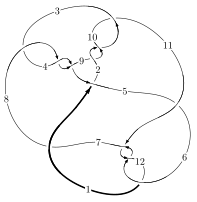
\includegraphics[width=112pt]{../../../GIT/diagram.site/Diagrams/png/2085_12a_1284.png}\\
\ \ \ A knot diagram\footnotemark}&
\allowdisplaybreaks
\textbf{Linearized knot diagam} \\
\cline{2-2}
 &
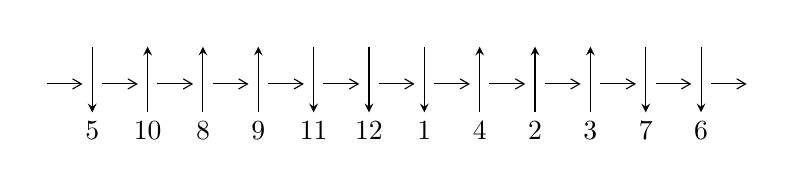
\begin{tikzpicture}[x=20pt, y=17pt]
	% nodes
	\node (C0) at (0, 0) {};
	\node (C1) at (1, 0) {};
	\node (C1U) at (1, +1) {};
	\node (C1D) at (1, -1) {5};

	\node (C2) at (2, 0) {};
	\node (C2U) at (2, +1) {};
	\node (C2D) at (2, -1) {10};

	\node (C3) at (3, 0) {};
	\node (C3U) at (3, +1) {};
	\node (C3D) at (3, -1) {8};

	\node (C4) at (4, 0) {};
	\node (C4U) at (4, +1) {};
	\node (C4D) at (4, -1) {9};

	\node (C5) at (5, 0) {};
	\node (C5U) at (5, +1) {};
	\node (C5D) at (5, -1) {11};

	\node (C6) at (6, 0) {};
	\node (C6U) at (6, +1) {};
	\node (C6D) at (6, -1) {12};

	\node (C7) at (7, 0) {};
	\node (C7U) at (7, +1) {};
	\node (C7D) at (7, -1) {1};

	\node (C8) at (8, 0) {};
	\node (C8U) at (8, +1) {};
	\node (C8D) at (8, -1) {4};

	\node (C9) at (9, 0) {};
	\node (C9U) at (9, +1) {};
	\node (C9D) at (9, -1) {2};

	\node (C10) at (10, 0) {};
	\node (C10U) at (10, +1) {};
	\node (C10D) at (10, -1) {3};

	\node (C11) at (11, 0) {};
	\node (C11U) at (11, +1) {};
	\node (C11D) at (11, -1) {7};

	\node (C12) at (12, 0) {};
	\node (C12U) at (12, +1) {};
	\node (C12D) at (12, -1) {6};
	\node (C13) at (13, 0) {};

	% arrows
	\draw[->,>={angle 60}]
	(C0) edge (C1) (C1) edge (C2) (C2) edge (C3) (C3) edge (C4) (C4) edge (C5) (C5) edge (C6) (C6) edge (C7) (C7) edge (C8) (C8) edge (C9) (C9) edge (C10) (C10) edge (C11) (C11) edge (C12) (C12) edge (C13) ;	\draw[->,>=stealth]
	(C1U) edge (C1D) (C2D) edge (C2U) (C3D) edge (C3U) (C4D) edge (C4U) (C5U) edge (C5D) (C6U) edge (C6D) (C7U) edge (C7D) (C8D) edge (C8U) (C9D) edge (C9U) (C10D) edge (C10U) (C11U) edge (C11D) (C12U) edge (C12D) ;
	\end{tikzpicture} \\
\hhline{~~} \\& 
\textbf{Solving Sequence} \\ \cline{2-2} 
 &
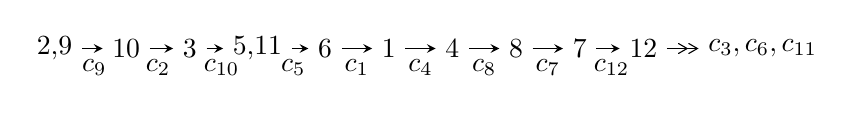
\begin{tikzpicture}[x=23pt, y=7pt]
	% node
	\node (A0) at (-1/8, 0) {2,9};
	\node (A1) at (1, 0) {10};
	\node (A2) at (2, 0) {3};
	\node (A3) at (49/16, 0) {5,11};
	\node (A4) at (33/8, 0) {6};
	\node (A5) at (41/8, 0) {1};
	\node (A6) at (49/8, 0) {4};
	\node (A7) at (57/8, 0) {8};
	\node (A8) at (65/8, 0) {7};
	\node (A9) at (73/8, 0) {12};
	\node (C1) at (1/2, -1) {$c_{9}$};
	\node (C2) at (3/2, -1) {$c_{2}$};
	\node (C3) at (5/2, -1) {$c_{10}$};
	\node (C4) at (29/8, -1) {$c_{5}$};
	\node (C5) at (37/8, -1) {$c_{1}$};
	\node (C6) at (45/8, -1) {$c_{4}$};
	\node (C7) at (53/8, -1) {$c_{8}$};
	\node (C8) at (61/8, -1) {$c_{7}$};
	\node (C9) at (69/8, -1) {$c_{12}$};
	\node (A10) at (11, 0) {$c_{3},c_{6},c_{11}$};

	% edge
	\draw[->,>=stealth]	
	(A0) edge (A1) (A1) edge (A2) (A2) edge (A3) (A3) edge (A4) (A4) edge (A5) (A5) edge (A6) (A6) edge (A7) (A7) edge (A8) (A8) edge (A9) ;
	\draw[->>,>={angle 60}]	
	(A9) edge (A10);
\end{tikzpicture} \\ 

\end{tabular} \\

\footnotetext{
The image of knot diagram is generated by the software ``\textbf{Draw programme}" developed by Andrew Bartholomew(\url{http://www.layer8.co.uk/maths/draw/index.htm\#Running-draw}), where we modified some parts for our purpose(\url{https://github.com/CATsTAILs/LinksPainter}).
}\phantom \\ \newline 
\centering \textbf{Ideals for irreducible components\footnotemark of $X_{\text{par}}$} 
 
\begin{align*}
I^u_{1}&=\langle 
b- u,\;u^{28}- u^{27}+\cdots+16 a-1,\;u^{30}- u^{29}+\cdots+2 u+1\rangle \\
I^u_{2}&=\langle 
6.24110\times10^{20} u^{39}+5.89445\times10^{20} u^{38}+\cdots+1.64141\times10^{21} b+4.89782\times10^{20},\\
\phantom{I^u_{2}}&\phantom{= \langle  }-1.01730\times10^{21} u^{39}+2.23086\times10^{21} u^{38}+\cdots+1.64141\times10^{21} a-2.79305\times10^{21},\;u^{40}- u^{39}+\cdots+2 u-1\rangle \\
I^u_{3}&=\langle 
b-1,\;a^4-3 a^2+3,\;u+1\rangle \\
I^u_{4}&=\langle 
b+1,\;a^4- a^2-1,\;u-1\rangle \\
I^u_{5}&=\langle 
b-1,\;a,\;u+1\rangle \\
\\
\end{align*}
\raggedright * 5 irreducible components of $\dim_{\mathbb{C}}=0$, with total 79 representations.\\
\footnotetext{All coefficients of polynomials are rational numbers. But the coefficients are sometimes approximated in decimal forms when there is not enough margin.}
\newpage
\renewcommand{\arraystretch}{1}
\centering \section*{I. $I^u_{1}= \langle b- u,\;u^{28}- u^{27}+\cdots+16 a-1,\;u^{30}- u^{29}+\cdots+2 u+1 \rangle$}
\flushleft \textbf{(i) Arc colorings}\\
\begin{tabular}{m{7pt} m{180pt} m{7pt} m{180pt} }
\flushright $a_{2}=$&$\begin{pmatrix}0\\u\end{pmatrix}$ \\
\flushright $a_{9}=$&$\begin{pmatrix}1\\0\end{pmatrix}$ \\
\flushright $a_{10}=$&$\begin{pmatrix}1\\- u^2\end{pmatrix}$ \\
\flushright $a_{3}=$&$\begin{pmatrix}u\\- u^3+u\end{pmatrix}$ \\
\flushright $a_{5}=$&$\begin{pmatrix}-0.0625000 u^{28}+0.0625000 u^{27}+\cdots+3.12500 u+0.0625000\\u\end{pmatrix}$ \\
\flushright $a_{11}=$&$\begin{pmatrix}- u^2+1\\u^4-2 u^2\end{pmatrix}$ \\
\flushright $a_{6}=$&$\begin{pmatrix}-0.0625000 u^{28}+0.0625000 u^{27}+\cdots+2.12500 u+0.0625000\\-\frac{1}{16} u^{28}+\frac{1}{16} u^{27}+\cdots+\frac{9}{8} u+\frac{1}{16}\end{pmatrix}$ \\
\flushright $a_{1}=$&$\begin{pmatrix}\frac{1}{16} u^{29}-\frac{1}{16} u^{28}+\cdots+\frac{3}{16} u+\frac{1}{8}\\-\frac{1}{16} u^{28}+\frac{1}{16} u^{27}+\cdots+\frac{9}{8} u+\frac{1}{16}\end{pmatrix}$ \\
\flushright $a_{4}=$&$\begin{pmatrix}-0.0625000 u^{28}+0.0625000 u^{27}+\cdots+2.12500 u+0.0625000\\u\end{pmatrix}$ \\
\flushright $a_{8}=$&$\begin{pmatrix}-\frac{1}{16} u^{29}+\frac{1}{16} u^{28}+\cdots+\frac{1}{16} u+1\\u^2\end{pmatrix}$ \\
\flushright $a_{7}=$&$\begin{pmatrix}\frac{11}{16} u^{29}-\frac{13}{16} u^{28}+\cdots-\frac{9}{16} u+\frac{5}{4}\\\frac{1}{16} u^{29}-\frac{1}{8} u^{28}+\cdots-\frac{1}{16} u+\frac{1}{16}\end{pmatrix}$ \\
\flushright $a_{12}=$&$\begin{pmatrix}-\frac{3}{16} u^{29}+\frac{7}{2} u^{27}+\cdots-\frac{5}{16} u-\frac{7}{16}\\-0.375000 u^{29}+0.937500 u^{28}+\cdots-0.250000 u-1.18750\end{pmatrix}$\\&\end{tabular}
\flushleft \textbf{(ii) Obstruction class $= -1$}\\~\\
\flushleft \textbf{(iii) Cusp Shapes $= \frac{5}{4} u^{29}-\frac{13}{8} u^{28}+\cdots+\frac{43}{4} u+\frac{33}{8}$}\\~\\
\newpage\renewcommand{\arraystretch}{1}
\flushleft \textbf{(iv) u-Polynomials at the component}\newline \\
\begin{tabular}{m{50pt}|m{274pt}}
Crossings & \hspace{64pt}u-Polynomials at each crossing \\
\hline $$\begin{aligned}c_{1}\end{aligned}$$&$\begin{aligned}
&u^{30}+21 u^{29}+\cdots-31648 u-3214
\end{aligned}$\\
\hline $$\begin{aligned}c_{2},c_{3},c_{4}\\c_{8},c_{9},c_{10}\end{aligned}$$&$\begin{aligned}
&u^{30}+u^{29}+\cdots-2 u+1
\end{aligned}$\\
\hline $$\begin{aligned}c_{5},c_{7}\end{aligned}$$&$\begin{aligned}
&u^{30}+3 u^{29}+\cdots-180 u-34
\end{aligned}$\\
\hline $$\begin{aligned}c_{6},c_{11},c_{12}\end{aligned}$$&$\begin{aligned}
&u^{30}-3 u^{29}+\cdots-7 u^2-2
\end{aligned}$\\
\hline
\end{tabular}\\~\\
\newpage\renewcommand{\arraystretch}{1}
\flushleft \textbf{(v) Riley Polynomials at the component}\newline \\
\begin{tabular}{m{50pt}|m{274pt}}
Crossings & \hspace{64pt}Riley Polynomials at each crossing \\
\hline $$\begin{aligned}c_{1}\end{aligned}$$&$\begin{aligned}
&y^{30}+5 y^{29}+\cdots+33781340 y+10329796
\end{aligned}$\\
\hline $$\begin{aligned}c_{2},c_{3},c_{4}\\c_{8},c_{9},c_{10}\end{aligned}$$&$\begin{aligned}
&y^{30}-37 y^{29}+\cdots-4 y+1
\end{aligned}$\\
\hline $$\begin{aligned}c_{5},c_{7}\end{aligned}$$&$\begin{aligned}
&y^{30}-19 y^{29}+\cdots+9692 y+1156
\end{aligned}$\\
\hline $$\begin{aligned}c_{6},c_{11},c_{12}\end{aligned}$$&$\begin{aligned}
&y^{30}+25 y^{29}+\cdots+28 y+4
\end{aligned}$\\
\hline
\end{tabular}\\~\\
\newpage\flushleft \textbf{(vi) Complex Volumes and Cusp Shapes}
$$\begin{array}{c|c|c}  
\text{Solutions to }I^u_{1}& \I (\text{vol} + \sqrt{-1}CS) & \text{Cusp shape}\\
 \hline 
\begin{aligned}
u &= -0.352980 + 0.621053 I \\
a &= -0.54691 + 1.67340 I \\
b &= -0.352980 + 0.621053 I\end{aligned}
 & \phantom{-}0.67916 - 7.00854 I & \phantom{-}0.01450 + 8.24477 I \\ \hline\begin{aligned}
u &= -0.352980 - 0.621053 I \\
a &= -0.54691 - 1.67340 I \\
b &= -0.352980 - 0.621053 I\end{aligned}
 & \phantom{-}0.67916 + 7.00854 I & \phantom{-}0.01450 - 8.24477 I \\ \hline\begin{aligned}
u &= \phantom{-}0.294160 + 0.620614 I \\
a &= \phantom{-}0.46496 + 1.62443 I \\
b &= \phantom{-}0.294160 + 0.620614 I\end{aligned}
 & -3.74541 + 3.07076 I & -5.43052 - 5.87151 I \\ \hline\begin{aligned}
u &= \phantom{-}0.294160 - 0.620614 I \\
a &= \phantom{-}0.46496 - 1.62443 I \\
b &= \phantom{-}0.294160 - 0.620614 I\end{aligned}
 & -3.74541 - 3.07076 I & -5.43052 + 5.87151 I \\ \hline\begin{aligned}
u &= -0.209229 + 0.628257 I \\
a &= -0.33328 + 1.58251 I \\
b &= -0.209229 + 0.628257 I\end{aligned}
 & -0.424922 + 0.787716 I & -2.53323 + 1.27592 I \\ \hline\begin{aligned}
u &= -0.209229 - 0.628257 I \\
a &= -0.33328 - 1.58251 I \\
b &= -0.209229 - 0.628257 I\end{aligned}
 & -0.424922 - 0.787716 I & -2.53323 - 1.27592 I \\ \hline\begin{aligned}
u &= \phantom{-}1.38964\phantom{ +0.000000I} \\
a &= -1.59527\phantom{ +0.000000I} \\
b &= \phantom{-}1.38964\phantom{ +0.000000I}\end{aligned}
 & \phantom{-}2.23351\phantom{ +0.000000I} & \phantom{-}3.74940\phantom{ +0.000000I} \\ \hline\begin{aligned}
u &= -1.391950 + 0.032239 I \\
a &= \phantom{-}1.56027 + 0.24632 I \\
b &= -1.391950 + 0.032239 I\end{aligned}
 & \phantom{-}6.15309 - 4.53590 I & \phantom{-}7.37130 + 3.41569 I \\ \hline\begin{aligned}
u &= -1.391950 - 0.032239 I \\
a &= \phantom{-}1.56027 - 0.24632 I \\
b &= -1.391950 - 0.032239 I\end{aligned}
 & \phantom{-}6.15309 + 4.53590 I & \phantom{-}7.37130 - 3.41569 I \\ \hline\begin{aligned}
u &= \phantom{-}0.416588 + 0.365315 I \\
a &= \phantom{-}0.98597 + 1.30700 I \\
b &= \phantom{-}0.416588 + 0.365315 I\end{aligned}
 & \phantom{-}5.06214 + 1.29762 I & \phantom{-}5.37578 - 5.33556 I\\
 \hline 
 \end{array}$$\newpage$$\begin{array}{c|c|c}  
\text{Solutions to }I^u_{1}& \I (\text{vol} + \sqrt{-1}CS) & \text{Cusp shape}\\
 \hline 
\begin{aligned}
u &= \phantom{-}0.416588 - 0.365315 I \\
a &= \phantom{-}0.98597 - 1.30700 I \\
b &= \phantom{-}0.416588 - 0.365315 I\end{aligned}
 & \phantom{-}5.06214 - 1.29762 I & \phantom{-}5.37578 + 5.33556 I \\ \hline\begin{aligned}
u &= -0.517665 + 0.077298 I \\
a &= -1.88180 + 0.43471 I \\
b &= -0.517665 + 0.077298 I\end{aligned}
 & \phantom{-}1.63781 + 3.82634 I & \phantom{-}1.68492 - 2.14247 I \\ \hline\begin{aligned}
u &= -0.517665 - 0.077298 I \\
a &= -1.88180 - 0.43471 I \\
b &= -0.517665 - 0.077298 I\end{aligned}
 & \phantom{-}1.63781 - 3.82634 I & \phantom{-}1.68492 + 2.14247 I \\ \hline\begin{aligned}
u &= \phantom{-}0.496783\phantom{ +0.000000I} \\
a &= \phantom{-}1.81590\phantom{ +0.000000I} \\
b &= \phantom{-}0.496783\phantom{ +0.000000I}\end{aligned}
 & -2.35493\phantom{ +0.000000I} & -2.87800\phantom{ +0.000000I} \\ \hline\begin{aligned}
u &= \phantom{-}1.49927 + 0.29227 I \\
a &= -0.387167 + 1.211670 I \\
b &= \phantom{-}1.49927 + 0.29227 I\end{aligned}
 & \phantom{-}10.74230 + 6.05762 I & \phantom{-}6.37484 - 2.22999 I \\ \hline\begin{aligned}
u &= \phantom{-}1.49927 - 0.29227 I \\
a &= -0.387167 - 1.211670 I \\
b &= \phantom{-}1.49927 - 0.29227 I\end{aligned}
 & \phantom{-}10.74230 - 6.05762 I & \phantom{-}6.37484 + 2.22999 I \\ \hline\begin{aligned}
u &= -1.51089 + 0.32477 I \\
a &= \phantom{-}0.274857 + 1.261600 I \\
b &= -1.51089 + 0.32477 I\end{aligned}
 & \phantom{-}8.04859 - 10.42510 I & \phantom{-}3.37060 + 6.14879 I \\ \hline\begin{aligned}
u &= -1.51089 - 0.32477 I \\
a &= \phantom{-}0.274857 - 1.261600 I \\
b &= -1.51089 - 0.32477 I\end{aligned}
 & \phantom{-}8.04859 + 10.42510 I & \phantom{-}3.37060 - 6.14879 I \\ \hline\begin{aligned}
u &= \phantom{-}1.53112 + 0.22334 I \\
a &= -0.460811 + 0.930719 I \\
b &= \phantom{-}1.53112 + 0.22334 I\end{aligned}
 & \phantom{-}11.80090 + 5.69316 I & \phantom{-}7.29124 - 4.91871 I \\ \hline\begin{aligned}
u &= \phantom{-}1.53112 - 0.22334 I \\
a &= -0.460811 - 0.930719 I \\
b &= \phantom{-}1.53112 - 0.22334 I\end{aligned}
 & \phantom{-}11.80090 - 5.69316 I & \phantom{-}7.29124 + 4.91871 I\\
 \hline 
 \end{array}$$\newpage$$\begin{array}{c|c|c}  
\text{Solutions to }I^u_{1}& \I (\text{vol} + \sqrt{-1}CS) & \text{Cusp shape}\\
 \hline 
\begin{aligned}
u &= -1.54555 + 0.16201 I \\
a &= \phantom{-}0.530144 + 0.687150 I \\
b &= -1.54555 + 0.16201 I\end{aligned}
 & \phantom{-}10.58750 - 1.81546 I & \phantom{-}5.41289 + 0. I\phantom{ +0.000000I} \\ \hline\begin{aligned}
u &= -1.54555 - 0.16201 I \\
a &= \phantom{-}0.530144 - 0.687150 I \\
b &= -1.54555 - 0.16201 I\end{aligned}
 & \phantom{-}10.58750 + 1.81546 I & \phantom{-}5.41289 + 0. I\phantom{ +0.000000I} \\ \hline\begin{aligned}
u &= \phantom{-}1.52517 + 0.34179 I \\
a &= -0.201317 + 1.264960 I \\
b &= \phantom{-}1.52517 + 0.34179 I\end{aligned}
 & \phantom{-}12.9098 + 14.6347 I & \phantom{-}7.58491 - 7.68189 I \\ \hline\begin{aligned}
u &= \phantom{-}1.52517 - 0.34179 I \\
a &= -0.201317 - 1.264960 I \\
b &= \phantom{-}1.52517 - 0.34179 I\end{aligned}
 & \phantom{-}12.9098 - 14.6347 I & \phantom{-}7.58491 + 7.68189 I \\ \hline\begin{aligned}
u &= -0.195804 + 0.351319 I \\
a &= -0.470190 + 1.033650 I \\
b &= -0.195804 + 0.351319 I\end{aligned}
 & -0.006279 - 0.796564 I & -0.20542 + 8.65055 I \\ \hline\begin{aligned}
u &= -0.195804 - 0.351319 I \\
a &= -0.470190 - 1.033650 I \\
b &= -0.195804 - 0.351319 I\end{aligned}
 & -0.006279 + 0.796564 I & -0.20542 - 8.65055 I \\ \hline\begin{aligned}
u &= \phantom{-}1.59665 + 0.14347 I \\
a &= -0.371698 + 0.545654 I \\
b &= \phantom{-}1.59665 + 0.14347 I\end{aligned}
 & \phantom{-}15.9724 - 1.4645 I & \phantom{-}10.01323 + 0. I\phantom{ +0.000000I} \\ \hline\begin{aligned}
u &= \phantom{-}1.59665 - 0.14347 I \\
a &= -0.371698 - 0.545654 I \\
b &= \phantom{-}1.59665 - 0.14347 I\end{aligned}
 & \phantom{-}15.9724 + 1.4645 I & \phantom{-}10.01323 + 0. I\phantom{ +0.000000I} \\ \hline\begin{aligned}
u &= -1.58211 + 0.26365 I \\
a &= \phantom{-}0.226662 + 0.948412 I \\
b &= -1.58211 + 0.26365 I\end{aligned}
 & \phantom{-}18.5173 - 6.9140 I & \phantom{-}11.23927 + 3.74532 I \\ \hline\begin{aligned}
u &= -1.58211 - 0.26365 I \\
a &= \phantom{-}0.226662 - 0.948412 I \\
b &= -1.58211 - 0.26365 I\end{aligned}
 & \phantom{-}18.5173 + 6.9140 I & \phantom{-}11.23927 - 3.74532 I\\
 \hline 
 \end{array}$$\newpage\newpage\renewcommand{\arraystretch}{1}
\centering \section*{II. $I^u_{2}= \langle 6.24\times10^{20} u^{39}+5.89\times10^{20} u^{38}+\cdots+1.64\times10^{21} b+4.90\times10^{20},\;-1.02\times10^{21} u^{39}+2.23\times10^{21} u^{38}+\cdots+1.64\times10^{21} a-2.79\times10^{21},\;u^{40}- u^{39}+\cdots+2 u-1 \rangle$}
\flushleft \textbf{(i) Arc colorings}\\
\begin{tabular}{m{7pt} m{180pt} m{7pt} m{180pt} }
\flushright $a_{2}=$&$\begin{pmatrix}0\\u\end{pmatrix}$ \\
\flushright $a_{9}=$&$\begin{pmatrix}1\\0\end{pmatrix}$ \\
\flushright $a_{10}=$&$\begin{pmatrix}1\\- u^2\end{pmatrix}$ \\
\flushright $a_{3}=$&$\begin{pmatrix}u\\- u^3+u\end{pmatrix}$ \\
\flushright $a_{5}=$&$\begin{pmatrix}0.619773 u^{39}-1.35911 u^{38}+\cdots+22.9232 u+1.70161\\-0.380227 u^{39}-0.359108 u^{38}+\cdots+4.92321 u-0.298390\end{pmatrix}$ \\
\flushright $a_{11}=$&$\begin{pmatrix}- u^2+1\\u^4-2 u^2\end{pmatrix}$ \\
\flushright $a_{6}=$&$\begin{pmatrix}0.543102 u^{39}-1.19599 u^{38}+\cdots+16.4379 u+1.69783\\-0.0232908 u^{39}-0.365372 u^{38}+\cdots+4.85714 u+0.0127958\end{pmatrix}$ \\
\flushright $a_{1}=$&$\begin{pmatrix}1.26580 u^{39}-1.30533 u^{38}+\cdots+27.7480 u+2.14255\\0.646027 u^{39}+0.0537756 u^{38}+\cdots+5.82476 u+0.440945\end{pmatrix}$ \\
\flushright $a_{4}=$&$\begin{pmatrix}u^{39}- u^{38}+\cdots+18 u+2\\-0.380227 u^{39}-0.359108 u^{38}+\cdots+4.92321 u-0.298390\end{pmatrix}$ \\
\flushright $a_{8}=$&$\begin{pmatrix}-0.298390 u^{39}-0.0818367 u^{38}+\cdots+15.7873 u+5.32643\\0.739335 u^{39}+0.286919 u^{38}+\cdots-0.462064 u+1.38023\end{pmatrix}$ \\
\flushright $a_{7}=$&$\begin{pmatrix}-0.525272 u^{39}-0.0557406 u^{38}+\cdots+1.36459 u-3.86438\\0.0790643 u^{39}+0.253718 u^{38}+\cdots+0.778092 u-0.531600\end{pmatrix}$ \\
\flushright $a_{12}=$&$\begin{pmatrix}0.268227 u^{39}-0.849361 u^{38}+\cdots+0.608273 u+1.83922\\0.302594 u^{39}+0.273543 u^{38}+\cdots+1.54337 u+0.135768\end{pmatrix}$\\&\end{tabular}
\flushleft \textbf{(ii) Obstruction class $= -1$}\\~\\
\flushleft \textbf{(iii) Cusp Shapes $= -\frac{6400585822088433349960}{1641414549632366281823} u^{39}-\frac{1917396265968610128824}{1641414549632366281823} u^{38}+\cdots-\frac{21817392701530411229944}{1641414549632366281823} u-\frac{8303876159610635920642}{1641414549632366281823}$}\\~\\
\newpage\renewcommand{\arraystretch}{1}
\flushleft \textbf{(iv) u-Polynomials at the component}\newline \\
\begin{tabular}{m{50pt}|m{274pt}}
Crossings & \hspace{64pt}u-Polynomials at each crossing \\
\hline $$\begin{aligned}c_{1}\end{aligned}$$&$\begin{aligned}
&(u^{20}-7 u^{19}+\cdots-6 u+1)^{2}
\end{aligned}$\\
\hline $$\begin{aligned}c_{2},c_{3},c_{4}\\c_{8},c_{9},c_{10}\end{aligned}$$&$\begin{aligned}
&u^{40}+u^{39}+\cdots-2 u-1
\end{aligned}$\\
\hline $$\begin{aligned}c_{5},c_{7}\end{aligned}$$&$\begin{aligned}
&(u^{20}- u^{19}+\cdots+4 u-1)^{2}
\end{aligned}$\\
\hline $$\begin{aligned}c_{6},c_{11},c_{12}\end{aligned}$$&$\begin{aligned}
&(u^{20}+u^{19}+\cdots+2 u-1)^{2}
\end{aligned}$\\
\hline
\end{tabular}\\~\\
\newpage\renewcommand{\arraystretch}{1}
\flushleft \textbf{(v) Riley Polynomials at the component}\newline \\
\begin{tabular}{m{50pt}|m{274pt}}
Crossings & \hspace{64pt}Riley Polynomials at each crossing \\
\hline $$\begin{aligned}c_{1}\end{aligned}$$&$\begin{aligned}
&(y^{20}+13 y^{19}+\cdots-6 y+1)^{2}
\end{aligned}$\\
\hline $$\begin{aligned}c_{2},c_{3},c_{4}\\c_{8},c_{9},c_{10}\end{aligned}$$&$\begin{aligned}
&y^{40}-33 y^{39}+\cdots-40 y+1
\end{aligned}$\\
\hline $$\begin{aligned}c_{5},c_{7}\end{aligned}$$&$\begin{aligned}
&(y^{20}-11 y^{19}+\cdots-6 y+1)^{2}
\end{aligned}$\\
\hline $$\begin{aligned}c_{6},c_{11},c_{12}\end{aligned}$$&$\begin{aligned}
&(y^{20}+17 y^{19}+\cdots-6 y+1)^{2}
\end{aligned}$\\
\hline
\end{tabular}\\~\\
\newpage\flushleft \textbf{(vi) Complex Volumes and Cusp Shapes}
$$\begin{array}{c|c|c}  
\text{Solutions to }I^u_{2}& \I (\text{vol} + \sqrt{-1}CS) & \text{Cusp shape}\\
 \hline 
\begin{aligned}
u &= \phantom{-}0.775780 + 0.647591 I \\
a &= -0.630465 - 0.581990 I \\
b &= -1.390130 + 0.052152 I\end{aligned}
 & \phantom{-}2.96536 - 0.81573 I & \phantom{-}2.32828 + 1.07888 I \\ \hline\begin{aligned}
u &= \phantom{-}0.775780 - 0.647591 I \\
a &= -0.630465 + 0.581990 I \\
b &= -1.390130 - 0.052152 I\end{aligned}
 & \phantom{-}2.96536 + 0.81573 I & \phantom{-}2.32828 - 1.07888 I \\ \hline\begin{aligned}
u &= -0.434102 + 0.914548 I \\
a &= \phantom{-}1.03581 - 1.10998 I \\
b &= \phantom{-}1.45939 - 0.21760 I\end{aligned}
 & \phantom{-}6.57229 - 10.05770 I & \phantom{-}5.29166 + 7.26612 I \\ \hline\begin{aligned}
u &= -0.434102 - 0.914548 I \\
a &= \phantom{-}1.03581 + 1.10998 I \\
b &= \phantom{-}1.45939 + 0.21760 I\end{aligned}
 & \phantom{-}6.57229 + 10.05770 I & \phantom{-}5.29166 - 7.26612 I \\ \hline\begin{aligned}
u &= -0.939888 + 0.425646 I \\
a &= \phantom{-}0.373710 - 0.231234 I \\
b &= \phantom{-}1.256600 + 0.168597 I\end{aligned}
 & \phantom{-}6.05405 - 2.16136 I & \phantom{-}7.26252 + 3.31855 I \\ \hline\begin{aligned}
u &= -0.939888 - 0.425646 I \\
a &= \phantom{-}0.373710 + 0.231234 I \\
b &= \phantom{-}1.256600 - 0.168597 I\end{aligned}
 & \phantom{-}6.05405 + 2.16136 I & \phantom{-}7.26252 - 3.31855 I \\ \hline\begin{aligned}
u &= \phantom{-}0.416544 + 0.869986 I \\
a &= -0.98007 - 1.14721 I \\
b &= -1.42778 - 0.21212 I\end{aligned}
 & \phantom{-}1.80703 + 6.07240 I & \phantom{-}0.54715 - 5.87540 I \\ \hline\begin{aligned}
u &= \phantom{-}0.416544 - 0.869986 I \\
a &= -0.98007 + 1.14721 I \\
b &= -1.42778 + 0.21212 I\end{aligned}
 & \phantom{-}1.80703 - 6.07240 I & \phantom{-}0.54715 + 5.87540 I \\ \hline\begin{aligned}
u &= \phantom{-}0.608596 + 0.846537 I \\
a &= -0.914359 - 0.871769 I \\
b &= -1.47424 - 0.09300 I\end{aligned}
 & \phantom{-}11.26460 + 2.84648 I & \phantom{-}9.60998 - 2.97861 I \\ \hline\begin{aligned}
u &= \phantom{-}0.608596 - 0.846537 I \\
a &= -0.914359 + 0.871769 I \\
b &= -1.47424 + 0.09300 I\end{aligned}
 & \phantom{-}11.26460 - 2.84648 I & \phantom{-}9.60998 + 2.97861 I\\
 \hline 
 \end{array}$$\newpage$$\begin{array}{c|c|c}  
\text{Solutions to }I^u_{2}& \I (\text{vol} + \sqrt{-1}CS) & \text{Cusp shape}\\
 \hline 
\begin{aligned}
u &= -0.946129 + 0.119622 I \\
a &= -1.166750 - 0.332930 I \\
b &= -0.126443 - 0.201400 I\end{aligned}
 & \phantom{-}1.63329 - 3.96853 I & \phantom{-}0.10651 + 3.79787 I \\ \hline\begin{aligned}
u &= -0.946129 - 0.119622 I \\
a &= -1.166750 + 0.332930 I \\
b &= -0.126443 + 0.201400 I\end{aligned}
 & \phantom{-}1.63329 + 3.96853 I & \phantom{-}0.10651 - 3.79787 I \\ \hline\begin{aligned}
u &= \phantom{-}0.916645\phantom{ +0.000000I} \\
a &= \phantom{-}1.24074\phantom{ +0.000000I} \\
b &= \phantom{-}0.149808\phantom{ +0.000000I}\end{aligned}
 & -2.26801\phantom{ +0.000000I} & -4.44030\phantom{ +0.000000I} \\ \hline\begin{aligned}
u &= -0.807999 + 0.735436 I \\
a &= \phantom{-}0.774534 - 0.558298 I \\
b &= \phantom{-}1.45140 + 0.05778 I\end{aligned}
 & \phantom{-}7.72048 + 4.43308 I & \phantom{-}7.31630 - 2.52728 I \\ \hline\begin{aligned}
u &= -0.807999 - 0.735436 I \\
a &= \phantom{-}0.774534 + 0.558298 I \\
b &= \phantom{-}1.45140 - 0.05778 I\end{aligned}
 & \phantom{-}7.72048 - 4.43308 I & \phantom{-}7.31630 + 2.52728 I \\ \hline\begin{aligned}
u &= -0.549205 + 0.695984 I \\
a &= \phantom{-}0.673732 - 0.972316 I \\
b &= \phantom{-}1.372450 - 0.086864 I\end{aligned}
 & \phantom{-}4.95641 - 2.35832 I & \phantom{-}5.64775 + 4.49783 I \\ \hline\begin{aligned}
u &= -0.549205 - 0.695984 I \\
a &= \phantom{-}0.673732 + 0.972316 I \\
b &= \phantom{-}1.372450 + 0.086864 I\end{aligned}
 & \phantom{-}4.95641 + 2.35832 I & \phantom{-}5.64775 - 4.49783 I \\ \hline\begin{aligned}
u &= -0.398694 + 0.774094 I \\
a &= \phantom{-}0.84367 - 1.21023 I \\
b &= \phantom{-}1.369530 - 0.189240 I\end{aligned}
 & \phantom{-}4.55875 - 2.13456 I & \phantom{-}3.49102 + 2.16962 I \\ \hline\begin{aligned}
u &= -0.398694 - 0.774094 I \\
a &= \phantom{-}0.84367 + 1.21023 I \\
b &= \phantom{-}1.369530 + 0.189240 I\end{aligned}
 & \phantom{-}4.55875 + 2.13456 I & \phantom{-}3.49102 - 2.16962 I \\ \hline\begin{aligned}
u &= -1.15120\phantom{ +0.000000I} \\
a &= -0.215264\phantom{ +0.000000I} \\
b &= \phantom{-}0.653394\phantom{ +0.000000I}\end{aligned}
 & \phantom{-}2.60969\phantom{ +0.000000I} & -2.76210\phantom{ +0.000000I}\\
 \hline 
 \end{array}$$\newpage$$\begin{array}{c|c|c}  
\text{Solutions to }I^u_{2}& \I (\text{vol} + \sqrt{-1}CS) & \text{Cusp shape}\\
 \hline 
\begin{aligned}
u &= \phantom{-}1.256600 + 0.168597 I \\
a &= -0.158159 + 0.320761 I \\
b &= -0.939888 + 0.425646 I\end{aligned}
 & \phantom{-}6.05405 - 2.16136 I & \phantom{-}7.26252 + 3.31855 I \\ \hline\begin{aligned}
u &= \phantom{-}1.256600 - 0.168597 I \\
a &= -0.158159 - 0.320761 I \\
b &= -0.939888 - 0.425646 I\end{aligned}
 & \phantom{-}6.05405 + 2.16136 I & \phantom{-}7.26252 - 3.31855 I \\ \hline\begin{aligned}
u &= \phantom{-}0.653394\phantom{ +0.000000I} \\
a &= \phantom{-}0.379269\phantom{ +0.000000I} \\
b &= -1.15120\phantom{ +0.000000I}\end{aligned}
 & \phantom{-}2.60969\phantom{ +0.000000I} & -2.76210\phantom{ +0.000000I} \\ \hline\begin{aligned}
u &= \phantom{-}1.372450 + 0.086864 I \\
a &= \phantom{-}0.176513 - 0.741916 I \\
b &= -0.549205 - 0.695984 I\end{aligned}
 & \phantom{-}4.95641 + 2.35832 I & \phantom{-0.000000 } 0 \\ \hline\begin{aligned}
u &= \phantom{-}1.372450 - 0.086864 I \\
a &= \phantom{-}0.176513 + 0.741916 I \\
b &= -0.549205 + 0.695984 I\end{aligned}
 & \phantom{-}4.95641 - 2.35832 I & \phantom{-0.000000 } 0 \\ \hline\begin{aligned}
u &= \phantom{-}1.369530 + 0.189240 I \\
a &= \phantom{-}0.317804 - 0.873099 I \\
b &= -0.398694 - 0.774094 I\end{aligned}
 & \phantom{-}4.55875 + 2.13456 I & \phantom{-0.000000 } 0 \\ \hline\begin{aligned}
u &= \phantom{-}1.369530 - 0.189240 I \\
a &= \phantom{-}0.317804 + 0.873099 I \\
b &= -0.398694 + 0.774094 I\end{aligned}
 & \phantom{-}4.55875 - 2.13456 I & \phantom{-0.000000 } 0 \\ \hline\begin{aligned}
u &= -1.390130 + 0.052152 I \\
a &= \phantom{-}0.057435 + 0.620642 I \\
b &= \phantom{-}0.775780 + 0.647591 I\end{aligned}
 & \phantom{-}2.96536 - 0.81573 I & \phantom{-0.000000 } 0 \\ \hline\begin{aligned}
u &= -1.390130 - 0.052152 I \\
a &= \phantom{-}0.057435 - 0.620642 I \\
b &= \phantom{-}0.775780 - 0.647591 I\end{aligned}
 & \phantom{-}2.96536 + 0.81573 I & \phantom{-0.000000 } 0 \\ \hline\begin{aligned}
u &= -1.42778 + 0.21212 I \\
a &= -0.268719 - 0.971795 I \\
b &= \phantom{-}0.416544 - 0.869986 I\end{aligned}
 & \phantom{-}1.80703 - 6.07240 I & \phantom{-0.000000 } 0\\
 \hline 
 \end{array}$$\newpage$$\begin{array}{c|c|c}  
\text{Solutions to }I^u_{2}& \I (\text{vol} + \sqrt{-1}CS) & \text{Cusp shape}\\
 \hline 
\begin{aligned}
u &= -1.42778 - 0.21212 I \\
a &= -0.268719 + 0.971795 I \\
b &= \phantom{-}0.416544 + 0.869986 I\end{aligned}
 & \phantom{-}1.80703 + 6.07240 I & \phantom{-0.000000 } 0 \\ \hline\begin{aligned}
u &= \phantom{-}1.45140 + 0.05778 I \\
a &= -0.120101 + 0.708049 I \\
b &= -0.807999 + 0.735436 I\end{aligned}
 & \phantom{-}7.72048 + 4.43308 I & \phantom{-0.000000 } 0 \\ \hline\begin{aligned}
u &= \phantom{-}1.45140 - 0.05778 I \\
a &= -0.120101 - 0.708049 I \\
b &= -0.807999 - 0.735436 I\end{aligned}
 & \phantom{-}7.72048 - 4.43308 I & \phantom{-0.000000 } 0 \\ \hline\begin{aligned}
u &= \phantom{-}1.45939 + 0.21760 I \\
a &= \phantom{-}0.236213 - 1.014500 I \\
b &= -0.434102 - 0.914548 I\end{aligned}
 & \phantom{-}6.57229 + 10.05770 I & \phantom{-0.000000 } 0 \\ \hline\begin{aligned}
u &= \phantom{-}1.45939 - 0.21760 I \\
a &= \phantom{-}0.236213 + 1.014500 I \\
b &= -0.434102 + 0.914548 I\end{aligned}
 & \phantom{-}6.57229 - 10.05770 I & \phantom{-0.000000 } 0 \\ \hline\begin{aligned}
u &= -1.47424 + 0.09300 I \\
a &= -0.067033 - 0.889156 I \\
b &= \phantom{-}0.608596 - 0.846537 I\end{aligned}
 & \phantom{-}11.26460 - 2.84648 I & \phantom{-0.000000 } 0 \\ \hline\begin{aligned}
u &= -1.47424 - 0.09300 I \\
a &= -0.067033 + 0.889156 I \\
b &= \phantom{-}0.608596 + 0.846537 I\end{aligned}
 & \phantom{-}11.26460 + 2.84648 I & \phantom{-0.000000 } 0 \\ \hline\begin{aligned}
u &= -0.126443 + 0.201400 I \\
a &= -3.18208 - 3.68109 I \\
b &= -0.946129 - 0.119622 I\end{aligned}
 & \phantom{-}1.63329 + 3.96853 I & \phantom{-}0.10651 - 3.79787 I \\ \hline\begin{aligned}
u &= -0.126443 - 0.201400 I \\
a &= -3.18208 + 3.68109 I \\
b &= -0.946129 + 0.119622 I\end{aligned}
 & \phantom{-}1.63329 - 3.96853 I & \phantom{-}0.10651 + 3.79787 I \\ \hline\begin{aligned}
u &= \phantom{-}0.149808\phantom{ +0.000000I} \\
a &= \phantom{-}7.59187\phantom{ +0.000000I} \\
b &= \phantom{-}0.916645\phantom{ +0.000000I}\end{aligned}
 & -2.26801\phantom{ +0.000000I} & -4.44030\phantom{ +0.000000I}\\
 \hline 
 \end{array}$$\newpage\newpage\renewcommand{\arraystretch}{1}
\centering \section*{III. $I^u_{3}= \langle b-1,\;a^4-3 a^2+3,\;u+1 \rangle$}
\flushleft \textbf{(i) Arc colorings}\\
\begin{tabular}{m{7pt} m{180pt} m{7pt} m{180pt} }
\flushright $a_{2}=$&$\begin{pmatrix}0\\-1\end{pmatrix}$ \\
\flushright $a_{9}=$&$\begin{pmatrix}1\\0\end{pmatrix}$ \\
\flushright $a_{10}=$&$\begin{pmatrix}1\\-1\end{pmatrix}$ \\
\flushright $a_{3}=$&$\begin{pmatrix}-1\\0\end{pmatrix}$ \\
\flushright $a_{5}=$&$\begin{pmatrix}a\\1\end{pmatrix}$ \\
\flushright $a_{11}=$&$\begin{pmatrix}0\\-1\end{pmatrix}$ \\
\flushright $a_{6}=$&$\begin{pmatrix}a\\a+1\end{pmatrix}$ \\
\flushright $a_{1}=$&$\begin{pmatrix}- a^2\\- a-1\end{pmatrix}$ \\
\flushright $a_{4}=$&$\begin{pmatrix}a-1\\1\end{pmatrix}$ \\
\flushright $a_{8}=$&$\begin{pmatrix}a\\1\end{pmatrix}$ \\
\flushright $a_{7}=$&$\begin{pmatrix}- a^3+a\\- a^2- a+1\end{pmatrix}$ \\
\flushright $a_{12}=$&$\begin{pmatrix}a^2-3\\a^3+2 a^2-2 a-4\end{pmatrix}$\\&\end{tabular}
\flushleft \textbf{(ii) Obstruction class $= 1$}\\~\\
\flushleft \textbf{(iii) Cusp Shapes $= 4 a^2$}\\~\\
\newpage\renewcommand{\arraystretch}{1}
\flushleft \textbf{(iv) u-Polynomials at the component}\newline \\
\begin{tabular}{m{50pt}|m{274pt}}
Crossings & \hspace{64pt}u-Polynomials at each crossing \\
\hline $$\begin{aligned}c_{1},c_{5},c_{7}\end{aligned}$$&$\begin{aligned}
&u^4-3 u^2+3
\end{aligned}$\\
\hline $$\begin{aligned}c_{2},c_{8}\end{aligned}$$&$\begin{aligned}
&(u-1)^4
\end{aligned}$\\
\hline $$\begin{aligned}c_{3},c_{4},c_{9}\\c_{10}\end{aligned}$$&$\begin{aligned}
&(u+1)^4
\end{aligned}$\\
\hline $$\begin{aligned}c_{6},c_{11},c_{12}\end{aligned}$$&$\begin{aligned}
&u^4+3 u^2+3
\end{aligned}$\\
\hline
\end{tabular}\\~\\
\newpage\renewcommand{\arraystretch}{1}
\flushleft \textbf{(v) Riley Polynomials at the component}\newline \\
\begin{tabular}{m{50pt}|m{274pt}}
Crossings & \hspace{64pt}Riley Polynomials at each crossing \\
\hline $$\begin{aligned}c_{1},c_{5},c_{7}\end{aligned}$$&$\begin{aligned}
&(y^2-3 y+3)^2
\end{aligned}$\\
\hline $$\begin{aligned}c_{2},c_{3},c_{4}\\c_{8},c_{9},c_{10}\end{aligned}$$&$\begin{aligned}
&(y-1)^4
\end{aligned}$\\
\hline $$\begin{aligned}c_{6},c_{11},c_{12}\end{aligned}$$&$\begin{aligned}
&(y^2+3 y+3)^2
\end{aligned}$\\
\hline
\end{tabular}\\~\\
\newpage\flushleft \textbf{(vi) Complex Volumes and Cusp Shapes}
$$\begin{array}{c|c|c}  
\text{Solutions to }I^u_{3}& \I (\text{vol} + \sqrt{-1}CS) & \text{Cusp shape}\\
 \hline 
\begin{aligned}
u &= -1.00000\phantom{ +0.000000I} \\
a &= \phantom{-}1.271230 + 0.340625 I \\
b &= \phantom{-}1.00000\phantom{ +0.000000I}\end{aligned}
 & \phantom{-}3.28987 - 4.05977 I & \phantom{-}6.00000 + 3.46410 I \\ \hline\begin{aligned}
u &= -1.00000\phantom{ +0.000000I} \\
a &= \phantom{-}1.271230 - 0.340625 I \\
b &= \phantom{-}1.00000\phantom{ +0.000000I}\end{aligned}
 & \phantom{-}3.28987 + 4.05977 I & \phantom{-}6.00000 - 3.46410 I \\ \hline\begin{aligned}
u &= -1.00000\phantom{ +0.000000I} \\
a &= -1.271230 + 0.340625 I \\
b &= \phantom{-}1.00000\phantom{ +0.000000I}\end{aligned}
 & \phantom{-}3.28987 + 4.05977 I & \phantom{-}6.00000 - 3.46410 I \\ \hline\begin{aligned}
u &= -1.00000\phantom{ +0.000000I} \\
a &= -1.271230 - 0.340625 I \\
b &= \phantom{-}1.00000\phantom{ +0.000000I}\end{aligned}
 & \phantom{-}3.28987 - 4.05977 I & \phantom{-}6.00000 + 3.46410 I\\
 \hline 
 \end{array}$$\newpage\newpage\renewcommand{\arraystretch}{1}
\centering \section*{IV. $I^u_{4}= \langle b+1,\;a^4- a^2-1,\;u-1 \rangle$}
\flushleft \textbf{(i) Arc colorings}\\
\begin{tabular}{m{7pt} m{180pt} m{7pt} m{180pt} }
\flushright $a_{2}=$&$\begin{pmatrix}0\\1\end{pmatrix}$ \\
\flushright $a_{9}=$&$\begin{pmatrix}1\\0\end{pmatrix}$ \\
\flushright $a_{10}=$&$\begin{pmatrix}1\\-1\end{pmatrix}$ \\
\flushright $a_{3}=$&$\begin{pmatrix}1\\0\end{pmatrix}$ \\
\flushright $a_{5}=$&$\begin{pmatrix}a\\-1\end{pmatrix}$ \\
\flushright $a_{11}=$&$\begin{pmatrix}0\\-1\end{pmatrix}$ \\
\flushright $a_{6}=$&$\begin{pmatrix}a\\a-1\end{pmatrix}$ \\
\flushright $a_{1}=$&$\begin{pmatrix}a^2\\- a+1\end{pmatrix}$ \\
\flushright $a_{4}=$&$\begin{pmatrix}a+1\\-1\end{pmatrix}$ \\
\flushright $a_{8}=$&$\begin{pmatrix}- a\\1\end{pmatrix}$ \\
\flushright $a_{7}=$&$\begin{pmatrix}a^3- a\\- a^2+a+1\end{pmatrix}$ \\
\flushright $a_{12}=$&$\begin{pmatrix}a^2-1\\a^3-2 a\end{pmatrix}$\\&\end{tabular}
\flushleft \textbf{(ii) Obstruction class $= 1$}\\~\\
\flushleft \textbf{(iii) Cusp Shapes $= -4 a^2+8$}\\~\\
\newpage\renewcommand{\arraystretch}{1}
\flushleft \textbf{(iv) u-Polynomials at the component}\newline \\
\begin{tabular}{m{50pt}|m{274pt}}
Crossings & \hspace{64pt}u-Polynomials at each crossing \\
\hline $$\begin{aligned}c_{1},c_{5},c_{7}\end{aligned}$$&$\begin{aligned}
&u^4- u^2-1
\end{aligned}$\\
\hline $$\begin{aligned}c_{2},c_{8}\end{aligned}$$&$\begin{aligned}
&(u+1)^4
\end{aligned}$\\
\hline $$\begin{aligned}c_{3},c_{4},c_{9}\\c_{10}\end{aligned}$$&$\begin{aligned}
&(u-1)^4
\end{aligned}$\\
\hline $$\begin{aligned}c_{6},c_{11},c_{12}\end{aligned}$$&$\begin{aligned}
&u^4+u^2-1
\end{aligned}$\\
\hline
\end{tabular}\\~\\
\newpage\renewcommand{\arraystretch}{1}
\flushleft \textbf{(v) Riley Polynomials at the component}\newline \\
\begin{tabular}{m{50pt}|m{274pt}}
Crossings & \hspace{64pt}Riley Polynomials at each crossing \\
\hline $$\begin{aligned}c_{1},c_{5},c_{7}\end{aligned}$$&$\begin{aligned}
&(y^2- y-1)^2
\end{aligned}$\\
\hline $$\begin{aligned}c_{2},c_{3},c_{4}\\c_{8},c_{9},c_{10}\end{aligned}$$&$\begin{aligned}
&(y-1)^4
\end{aligned}$\\
\hline $$\begin{aligned}c_{6},c_{11},c_{12}\end{aligned}$$&$\begin{aligned}
&(y^2+y-1)^2
\end{aligned}$\\
\hline
\end{tabular}\\~\\
\newpage\flushleft \textbf{(vi) Complex Volumes and Cusp Shapes}
$$\begin{array}{c|c|c}  
\text{Solutions to }I^u_{4}& \I (\text{vol} + \sqrt{-1}CS) & \text{Cusp shape}\\
 \hline 
\begin{aligned}
u &= \phantom{-}1.00000\phantom{ +0.000000I} \\
a &= \phantom{-0.000000 -}0.786151 I \\
b &= -1.00000\phantom{ +0.000000I}\end{aligned}
 & \phantom{-}7.23771\phantom{ +0.000000I} & \phantom{-}10.4720\phantom{ +0.000000I} \\ \hline\begin{aligned}
u &= \phantom{-}1.00000\phantom{ +0.000000I} \\
a &= \phantom{-0.000000 } -0.786151 I \\
b &= -1.00000\phantom{ +0.000000I}\end{aligned}
 & \phantom{-}7.23771\phantom{ +0.000000I} & \phantom{-}10.4720\phantom{ +0.000000I} \\ \hline\begin{aligned}
u &= \phantom{-}1.00000\phantom{ +0.000000I} \\
a &= \phantom{-}1.27202\phantom{ +0.000000I} \\
b &= -1.00000\phantom{ +0.000000I}\end{aligned}
 & -0.657974\phantom{ +0.000000I} & \phantom{-}1.52790\phantom{ +0.000000I} \\ \hline\begin{aligned}
u &= \phantom{-}1.00000\phantom{ +0.000000I} \\
a &= -1.27202\phantom{ +0.000000I} \\
b &= -1.00000\phantom{ +0.000000I}\end{aligned}
 & -0.657974\phantom{ +0.000000I} & \phantom{-}1.52790\phantom{ +0.000000I}\\
 \hline 
 \end{array}$$\newpage\newpage\renewcommand{\arraystretch}{1}
\centering \section*{V. $I^u_{5}= \langle b-1,\;a,\;u+1 \rangle$}
\flushleft \textbf{(i) Arc colorings}\\
\begin{tabular}{m{7pt} m{180pt} m{7pt} m{180pt} }
\flushright $a_{2}=$&$\begin{pmatrix}0\\-1\end{pmatrix}$ \\
\flushright $a_{9}=$&$\begin{pmatrix}1\\0\end{pmatrix}$ \\
\flushright $a_{10}=$&$\begin{pmatrix}1\\-1\end{pmatrix}$ \\
\flushright $a_{3}=$&$\begin{pmatrix}-1\\0\end{pmatrix}$ \\
\flushright $a_{5}=$&$\begin{pmatrix}0\\1\end{pmatrix}$ \\
\flushright $a_{11}=$&$\begin{pmatrix}0\\-1\end{pmatrix}$ \\
\flushright $a_{6}=$&$\begin{pmatrix}0\\1\end{pmatrix}$ \\
\flushright $a_{1}=$&$\begin{pmatrix}0\\-1\end{pmatrix}$ \\
\flushright $a_{4}=$&$\begin{pmatrix}-1\\1\end{pmatrix}$ \\
\flushright $a_{8}=$&$\begin{pmatrix}0\\1\end{pmatrix}$ \\
\flushright $a_{7}=$&$\begin{pmatrix}0\\1\end{pmatrix}$ \\
\flushright $a_{12}=$&$\begin{pmatrix}0\\-1\end{pmatrix}$\\&\end{tabular}
\flushleft \textbf{(ii) Obstruction class $= 1$}\\~\\
\flushleft \textbf{(iii) Cusp Shapes $= 12$}\\~\\
\newpage\renewcommand{\arraystretch}{1}
\flushleft \textbf{(iv) u-Polynomials at the component}\newline \\
\begin{tabular}{m{50pt}|m{274pt}}
Crossings & \hspace{64pt}u-Polynomials at each crossing \\
\hline $$\begin{aligned}c_{1},c_{5},c_{6}\\c_{7},c_{11},c_{12}\end{aligned}$$&$\begin{aligned}
&u
\end{aligned}$\\
\hline $$\begin{aligned}c_{2},c_{8}\end{aligned}$$&$\begin{aligned}
&u-1
\end{aligned}$\\
\hline $$\begin{aligned}c_{3},c_{4},c_{9}\\c_{10}\end{aligned}$$&$\begin{aligned}
&u+1
\end{aligned}$\\
\hline
\end{tabular}\\~\\
\newpage\renewcommand{\arraystretch}{1}
\flushleft \textbf{(v) Riley Polynomials at the component}\newline \\
\begin{tabular}{m{50pt}|m{274pt}}
Crossings & \hspace{64pt}Riley Polynomials at each crossing \\
\hline $$\begin{aligned}c_{1},c_{5},c_{6}\\c_{7},c_{11},c_{12}\end{aligned}$$&$\begin{aligned}
&y
\end{aligned}$\\
\hline $$\begin{aligned}c_{2},c_{3},c_{4}\\c_{8},c_{9},c_{10}\end{aligned}$$&$\begin{aligned}
&y-1
\end{aligned}$\\
\hline
\end{tabular}\\~\\
\newpage\flushleft \textbf{(vi) Complex Volumes and Cusp Shapes}
$$\begin{array}{c|c|c}  
\text{Solutions to }I^u_{5}& \I (\text{vol} + \sqrt{-1}CS) & \text{Cusp shape}\\
 \hline 
\begin{aligned}
u &= -1.00000\phantom{ +0.000000I} \\
a &= \phantom{-0.000000 } 0 \\
b &= \phantom{-}1.00000\phantom{ +0.000000I}\end{aligned}
 & \phantom{-}3.28987\phantom{ +0.000000I} & \phantom{-}12.0000\phantom{ +0.000000I}\\
 \hline 
 \end{array}$$\newpage
\newpage\renewcommand{\arraystretch}{1}
\centering \section*{ VI. u-Polynomials}
\begin{tabular}{m{50pt}|m{274pt}}
Crossings & \hspace{64pt}u-Polynomials at each crossing \\
\hline $$\begin{aligned}c_{1}\end{aligned}$$&$\begin{aligned}
&u(u^4-3 u^2+3)(u^4- u^2-1)(u^{20}-7 u^{19}+\cdots-6 u+1)^{2}\\
&\cdot(u^{30}+21 u^{29}+\cdots-31648 u-3214)
\end{aligned}$\\
\hline $$\begin{aligned}c_{2},c_{8}\end{aligned}$$&$\begin{aligned}
&((u-1)^5)(u+1)^4(u^{30}+u^{29}+\cdots-2 u+1)(u^{40}+u^{39}+\cdots-2 u-1)
\end{aligned}$\\
\hline $$\begin{aligned}c_{3},c_{4},c_{9}\\c_{10}\end{aligned}$$&$\begin{aligned}
&((u-1)^4)(u+1)^5(u^{30}+u^{29}+\cdots-2 u+1)(u^{40}+u^{39}+\cdots-2 u-1)
\end{aligned}$\\
\hline $$\begin{aligned}c_{5},c_{7}\end{aligned}$$&$\begin{aligned}
&u(u^4-3 u^2+3)(u^4- u^2-1)(u^{20}- u^{19}+\cdots+4 u-1)^{2}\\
&\cdot(u^{30}+3 u^{29}+\cdots-180 u-34)
\end{aligned}$\\
\hline $$\begin{aligned}c_{6},c_{11},c_{12}\end{aligned}$$&$\begin{aligned}
&u(u^4+u^2-1)(u^4+3 u^2+3)(u^{20}+u^{19}+\cdots+2 u-1)^{2}\\
&\cdot(u^{30}-3 u^{29}+\cdots-7 u^2-2)
\end{aligned}$\\
\hline
\end{tabular}\newpage\renewcommand{\arraystretch}{1}
\centering \section*{ VII. Riley Polynomials}
\begin{tabular}{m{50pt}|m{274pt}}
Crossings & \hspace{64pt}Riley Polynomials at each crossing \\
\hline $$\begin{aligned}c_{1}\end{aligned}$$&$\begin{aligned}
&y(y^2-3 y+3)^2(y^2- y-1)^2(y^{20}+13 y^{19}+\cdots-6 y+1)^{2}\\
&\cdot(y^{30}+5 y^{29}+\cdots+33781340 y+10329796)
\end{aligned}$\\
\hline $$\begin{aligned}c_{2},c_{3},c_{4}\\c_{8},c_{9},c_{10}\end{aligned}$$&$\begin{aligned}
&((y-1)^9)(y^{30}-37 y^{29}+\cdots-4 y+1)(y^{40}-33 y^{39}+\cdots-40 y+1)
\end{aligned}$\\
\hline $$\begin{aligned}c_{5},c_{7}\end{aligned}$$&$\begin{aligned}
&y(y^2-3 y+3)^2(y^2- y-1)^2(y^{20}-11 y^{19}+\cdots-6 y+1)^{2}\\
&\cdot(y^{30}-19 y^{29}+\cdots+9692 y+1156)
\end{aligned}$\\
\hline $$\begin{aligned}c_{6},c_{11},c_{12}\end{aligned}$$&$\begin{aligned}
&y(y^2+y-1)^2(y^2+3 y+3)^2(y^{20}+17 y^{19}+\cdots-6 y+1)^{2}\\
&\cdot(y^{30}+25 y^{29}+\cdots+28 y+4)
\end{aligned}$\\
\hline
\end{tabular}
\vskip 2pc
\end{document}